\documentclass[../../main.tex]{subfiles}

\begin{document}

\label{sec:abbildungen_symmetrie}

Die wichtigsten Symmetrien, die du aus den Grundlagen der Geometrie kennst, sind Spiegelungen und Drehungen. Nachfolgend geht es darum, Spiegelungen bei Abbildungsgraphen zu suchen.

Wenn man davon spricht, dass der Graph einer Abbildung symmetrisch ist, dann meint man normalerweise \enquote{symmetrisch am Ursprung} oder \enquote{symmetrisch an der $y$-Achse}. Prinzipiell heißt das, dass der Graph links von der $y$-Achse auf die gleiche Weise verläuft wie rechts von der $y$-Achse.

\begin{advanced}{Symmetrien}
    Man kann auch allgemeiner Symmetrien statt nur Spiegelungen bei Abbildungsgraphen suchen. Eine \textbf{Symmetrie} ist eine Abbildung, die die Punkte einer geometrischen Figur (also zum Beispiel die Punkte auf einem Abbildungsgraphen) umordnet und dabei Abstände beibehält. Zwei Punkte, die einen Abstand von 1 haben, müssen durch eine Symmetrie demnach auf zwei Punkte abgebildet werden, deren Abstand ebenfalls 1 ist.
    
    \begin{definition}{Symmetrie}
        Es sei $F$ eine geometrische Figur, dargestellt durch die Menge der Punkte, die zur Figur gehören. Dann heißt eine bijektive Abbildung $s\colon F\rightarrow F$ eine Symmetrie von $F$, falls beliebige $f_1,f_2\in F$ stets denselben Abstand wie $s(f_1)$ und $s(f_2)$ haben.
    \end{definition}
    
    \begin{advexample}{}
        \parpic[r]{
            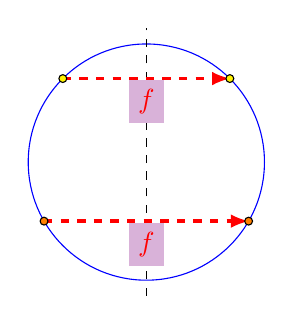
\begin{tikzpicture}
                \draw[blue] (0,0) circle[radius=1.5cm];
                \draw[dashed] (0,-1.7) -- (0,1.7);
                \draw[very thick,-latex,dashed,red] (135:1.5) -- node[fill=violet!30,below] {$f$} (45:1.5);
                \draw[very thick,-latex,dashed,red] (-150:1.5) -- node[fill=violet!30,below] {$f$} (-30:1.5);
                \draw[fill=yellow] (45:1.5) circle[radius=.5mm];
                \draw[fill=yellow] (135:1.5) circle[radius=.5mm];
                \draw[fill=orange] (-30:1.5) circle[radius=.5mm];
                \draw[fill=orange] (-150:1.5) circle[radius=.5mm];
            \end{tikzpicture}
        }
        Eine Symmetrie des rechts abgebildeten blauen Kreises ist die eingezeichnete Abbildung, die jeden Punkt des Kreises an der gestrichelt eingezeichneten Spiegelachse spiegelt.
        
        Nach der Anwendung der Spiegelung erhält man d\textbf{en gleichen Kreis wie vorher}. Außerdem haben zwei Punkte vor der Spiegelung immer den \textbf{gleichen Abstand} wie nach der Spiegelung. Diese beiden Eigenschaften machen die eingezeichnete Abbildung zu einer Symmetrie.
        
        Eine weitere Symmetrie des Kreises ist eine Abbildung, die jeden Punkt auf sich selbst abbildet. Diese Symmetrie existiert bei jeder geometrischen Figur und behält natürlich auch die Abstände bei, weil sie die Punkte nicht verschiebt.
    \end{advexample}
\end{advanced}

\begin{example}{}
    \parpic[r]{
        \begin{tikzpicture}
            \begin{axis}[defgrid, domain=-2:2, y=.75cm, x=.75cm, xtick={-2,...,2}, ytick={1,2,3}, samples=\ifdraft{5}{20}]
                \addplot[color=violet] expression{x^2-1};
            \end{axis}
        \end{tikzpicture}
    }
    Der rechts abgebildete Graph, der durch die Berechnungsvorschrift $f(x)=x^2-1$ entsteht, verläuft links von der $y$-Achse genauso wie rechts von von der $y$-Achse: Egal, ob man dem Graphen von der $y$-Achse nach links oder rechts folgt, seine $y$-Werte entwickeln sich immer gleich.
    
    Man sieht, dass der Graph achsensymmetrisch an der $y$-Achse ist (man nutzt die $y$-Achse also als Spiegelachse).
\end{example}

Der Graph aus dem letzten Beispiel ist \textbf{achsensymmetrisch an der $y$-Achse}. Das heißt, dass die $y$-Achse als Spiegelachse fungiert und sich der Teil links von der $y$-Achse auf den Teil rechts von der $y$-Achse klappen lässt.


\parpic[r]{
    \begin{tikzpicture}
        \begin{axis}[defgrid, domain=-2:2, y=1cm, x=1cm, xtick={-2,...,2}, ytick={1,2,3}, yticklabels={~,~,3},ymax=3]
            \addplot[mark=*, only marks, fill=white] coordinates {(-1,2) (1, 2)};
            \addplot[mark=*, only marks, fill=yellow] coordinates {(-2,1) (2, 1)};
            \draw[very thick,-latex,red,dashed] (-2,1) -- (2,1);
            \draw[very thick,-latex,red,dashed] (-1,2) -- (1,2);
        \end{axis}
    \end{tikzpicture}
}
Nutzt man die $y$-Achse als Spiegelachse, dann werden alle Punkte auf der linken Seite (also mit negativen $x$-Werten) in gerader Linie nach rechts gespiegelt. Der gelbe Punkt auf der linken Seite wird in waagerechter Linie nach rechts gespiegelt. Dadurch verändert sich sein $y$-Wert nicht. Durch die Spiegelung ändert sich das Vorzeichen der $x$-Koordinate, weil der Punkt nach der Spiegelung genauso weit rechts von der $y$-Achse ist wie er vorher links war.

Das bedeutet auch, dass man die gleichen Funktionswerte erhält, egal ob man von der $y$-Achse eine gewisse Schrittzahl nach links oder rechts geht: Letztendlich verläuft der Graph auf beiden Seiten auf der gleichen Höhe.

\begin{example}{}
    \parpic[r]{
        \begin{tikzpicture}
            \begin{axis}[defgrid, domain=-2:2, y=.75cm, x=.75cm, xtick={-2,...,2}, ytick={1,2}, samples=\ifdraft{5}{20}]
                \addplot[color=violet] expression{x^2-1};
                \addplot[mark=*, only marks, fill=white] coordinates {(-1,0) (1, 0)};
                \addplot[mark=*, only marks, fill=yellow] coordinates {(-2,3) (2, 3)};
                \draw[very thick,-latex,dashed] (-2,3) -- (2,3);
            \end{axis}
        \end{tikzpicture}
    }
    Geht man im letzten Beispiel vom Ursprung einen Schritt auf der $x$-Achse nach links, so schneidet der Graph dort beim Punkt $\coord{-1}{0}$ die $x$-Achse (dargestellt durch weiße Punkte, es gilt $f(-1)=0$). Wenn du dir vorstellst, dass du den Punkt $\coord{-1}{0}$ nun nach rechts spiegelst, dann bekommst du den Punkt $\coord{1}{0}$, der ebenfalls auf dem Graphen liegt. Dieser Punkt stellt die Regel $f(1)=0$ dar.
    
    \picskip{0}
    Wenn man zwei Schritte nach links oder rechts geht (also zu $x=-2$ oder $x=2$), dann findet man für jeden dieser $x$-Werte einen Punkt auf dem Graphen (dargestellt durch die gelben Punkte). Die Punkte haben die Koordinaten $\coord{-2}{3}$ und $\coord{2}{3}$, stellen also die Abbildungsregeln $f(-2)=3$ und $f(2)=3$ dar.
\end{example}

Im letzten Beispiel konnte beobachtet werden, dass ein beliebiger Punkt $\coord{x}{y}$ auf dem Graphen bei der Achsenspiegelung an der $y$-Achse auf den Punkt $\coord{-x}{y}$ gespiegelt wird. Das heißt, dass zu einem Graphen, der achsensymmetrisch an der $y$-Achse ist und den Punkt $\coord{x}{y}$ enthält, auch immer der Punkt $\coord{-x}{y}$ gehören muss.

Wenn der Punkt $\coord{x}{y}$ auf dem Graphen einer Abbildung liegt, dann steht das immer für die Abbildungsregel $f(x)=y$. Der gespiegelte Punkt steht also für die Regel $f(-x)=y$. Damit ist insgesamt $f(x)=f(-x)$ (denn beides hat denselben Wert, nämlich $y$). Abbildungen, deren Graph achsensymmetrisch an der $y$-Achse ist, haben also die Eigenschaft, dass $f(x)=f(-x)$ ist.

\begin{theorem}{}
    Der Graph einer Abbildung $f$ ist genau dann achsensymmetrisch an der $y$-Achse, wenn $f(x)=f(-x)$ für alle $x\in\Real$ gilt.
\end{theorem}

\begin{example}{}
    Es lässt sich rechnerisch erklären, dass der Graph der Abbildung $f(x)=x^2-1$ achsensymmetrisch an der $y$-Achse ist: Es gilt \[f(-x)=(-x)^2-1=x^2-1=f(x),\] also insgesamt $f(x)=f(-x)$. Die Bedingung $f(x)=f(-x)$ ist nach den vorherigen Überlegungen genau die Voraussetzung für die Achsensymmetrie an der $y$-Achse.
\end{example}

Anders als in den vorherigen Beispielen ist es auch möglich, dass der Graph nicht an der $y$-Achse achsengespiegelt ist, sondern stattdessen punktgespiegelt am Ursprung. Dabei wird der Graph nicht einfach von links nach rechts geklappt.

\begin{example}{}
    \parpic[r]{
        \begin{tikzpicture}
            \begin{axis}[defgrid, domain=-2:2, y=.75cm, x=.75cm, xtick={-2,-1,1,2}, xticklabels={-2,~,1,2}, ytick={-4,...,4}, samples=\ifdraft{5}{20}]
                \addplot[color=violet] expression{0.5*x^3};
                \addplot[mark=*, only marks, fill=white] coordinates {(-1.5,-1.6875)};
                \addplot[mark=*, only marks, fill=yellow] coordinates {(1.5, 1.6875)};
                \draw[very thick,dashed,-latex] (-1.5,-1.6875) -- (1.5,1.6875);
            \end{axis}
        \end{tikzpicture}
    }
    Der Graph, den du rechts siehst, ist punktsymmetrisch. Spiegelt man zum Beispiel den weiß eingezeichneten Punkt, der bei der $x$-Koordinate $-\frac{3}{2}$ liegt, am Ursprung, dann landet man beim gelb eingezeichneten Punkt genau auf der anderen Seite.
    
    Auf die gleiche Weise wie den weißen Punkt könnte man jeden anderen Punkt vom Graphen am Ursprung spiegeln und würde jedes Mal wieder auf dem Graphen landen.
    
    War der Punkt vor der Punktspiegelung links von der $y$-Achse, so ist er anschließend rechts. Die $x$-Koordinate verändert sich wie bereits bei der Achsenspiegelung nur, indem es aus positiven Koordinaten negative werden und umgekehrt.
\end{example}

Die Punktspiegelung am Ursprung ähnelt sehr der Achsenspiegelung an der $y$-Achse: Bei der Spiegelung werden Punkte von links nach rechts (oder umgekehrt) gespiegelt. Der wesentliche Unterschied ist allerdings, dass die Spiegelung vorher in einer waagerechten Linie erfolgt ist. Hatte ein Punkt vor der Achsenspiegelung zum Beispiel die $y$-Koordinate $6$, so behält er diese Koordinate auch nach der Spiegelung.

Das ist nun anders: Punkte werden hier auch nach oben (oder unten, falls sie bereits oben waren) gespiegelt. Dadurch verändert sich bei der Spiegelung nun nicht nur die $x$-Koordinate, sondern dasselbe passiert nun auch mit der $y$-Koordinate.

Spiegeln wir etwa den Punkt $\coord{-2}{-2}$ am Ursprung, dann liegt der gespiegelte Punkt anschließend genauso weit rechts und oben wie der ursprüngliche Punkt links und unten lag. Mit anderen Worten: Bei der $x$- und der $y$-Koordinate ändert sich jeweils das Vorzeichen. Der neue Punkt lautet in diesem Fall $\coord{2}{2}$.

Liegt nun ein Punkt $\coord{x}{y}$ auf dem Abbildungsgraphen (das stellt die Regel $f(x)=y$ dar), dann liegt ebenso sein gespiegelter Punkt auf dem Graphen. Dieser hat nach den vorherigen Überlegungen die Koordinaten $\coord{-x}{-y}$ und stellt damit die Abbildungsregel $f(-x)=-y$ dar. Für jede Abbildungsregel $f(x)=y$ lässt sich demnach sofort feststellen, dass auch $f(-x)=-y$ eine Regel sein muss (denn der entsprechende Punkt liegt auf dem Graphen). Formen wir diese Bedingung ein wenig um, dann erhalten wir \[f(x)=y=-(-y)=-f(-x),\]
also hat eine Abbildung einen punktsymmetrischen Graphen, falls stets $f(x)=-f(-x)$ gilt.

\begin{theorem}{}
    Der Graph einer Abbildung $f$ ist genau dann punktsymmetrisch am Ursprung, wenn $f(x)=-f(-x)$ für alle $x\in\Real$ gilt.
\end{theorem}

\begin{example}{}
    Der Graph der Abbildung $f(x)=x^3$ ist punktsymmetrisch am Ursprung. Um zu prüfen, ob der Graph punktsymmetrisch ist, muss geschaut werden, ob \mbox{$f(x)=-f(-x)$} gilt. Weil $f(x)$ nichts anderes als $x^3$ ist, muss hier lediglich geprüft werden, ob $x^3$ dasselbe ist wie $-\colorbrace{(-x)^3}{f(-x)}$. Wir können nun leicht nachrechnen, dass
    \[-(-x)^3=-(-x^3)=x^3\]
    gilt. Und das ist genau dasselbe wie $f(x)$. Der Graph der Funktion ist also punktsymmetrisch am Ursprung.
\end{example}

\begin{nutshell}{Symmetrie bei Abbildungsgraphen}
    Einige Abbildungen haben Graphen, die entweder punkt-- oder achsensymmetrisch sind. Man unterscheidet zwischen Graphen, die achsensymmetrisch an der $y$-Achse sind und Graphen, die punktsymmetrisch am Ursprung sind.
    
    Bei einer \textbf{Spiegelung an der $y$-Achse} werden alle Punkte wagerecht von links nach rechts (oder andersrum) geklappt. Damit ein Graph achsensymmetrisch an der $y$-Achse ist, muss $f(x)=f(-x)$ gelten (d.h. er verläuft links der $y$-Achse ebenso wie rechts von der $y$-Achse).
    
    Für eine \textbf{Punktspiegelung am Ursprung} werden Punkte diagonal gespiegelt. Ein am Ursprung punktgespiegelter Graph verläuft links genauso wie rechts, allerdings mit einem Vorzeichenwechsel. Verläuft er links nach unten, dann verläuft der Graph rechts nach oben. Es liegt eine Punktsymmetrie am Ursprung vor, wenn $f(x)=-f(-x)$ gilt.
\end{nutshell}


\end{document}